\documentclass[a4paper, 12pt]{scrreprt} 

    \usepackage{cmap}
    \usepackage{graphicx} 
    \usepackage{wrapfig}
    \usepackage{lastpage}
    \usepackage{tikz}
    \usepackage{pgfplots}
    \usepackage{braket}
    \usepackage{verbatim}
    \usetikzlibrary{arrows}
    \usetikzlibrary{calc,positioning,fit,backgrounds}
    \usetikzlibrary{decorations.pathreplacing,calc}
    \usepackage{amsmath} 
    \usepackage{color}
    \usepackage[T2A]{fontenc}
    \usepackage[utf8]{inputenc}	
    \usepackage[english,russian]{babel}
    \usepackage{geometry} 
    \geometry{top=25mm}
    \geometry{bottom=25mm}
    \geometry{left=16mm}
    \geometry{right=16mm}	
    \usepackage{amssymb}
    \usepackage{icomma} 
    \usepackage{mathtext} 
    \usepackage{mathrsfs}
    \usepackage{mathtools}
    \usepackage{fancyhdr}
    \usepackage{mdframed}
    \newmdenv[
  topline=false,
  bottomline=false,
  skipabove=\topsep,
  skipbelow=\topsep,
  leftmargin=20pt,
  rightmargin=20pt,
  innertopmargin=0pt,
  innerbottommargin=0pt
]{siderules}
    %\pagestyle{fancy}
    %\fancyhf{}
    %\renewcommand{\headrulewidth}{0,04mm}
    \usepackage{hyperref}
    \usepackage{mathtext} 
    \usepackage{multicol}
    %\rhead{\scshape{BEC 171}}
    %\lhead{\scshape{Research seminar for research stream}}
    %\chead{} 
    \cfoot{\thepage} 
    \hypersetup{
      colorlinks=true
       linkcolor=red,       
            citecolor=black,   
            filecolor=magenta,  
            urlcolor=blue}
    \makeatletter 
    \renewcommand{\headrulewidth}{0,4mm} 
    %ЦВЕТА
    \newcommand{\blue}[1]{\textcolor[rgb]{.4,.2,.4}{#1}}
    \newcommand{\ot}[1]{\textcolor[rgb]{.55,.45,.55}{#1}}
    \newcommand{\oq}[1]{\textcolor[rgb]{.8,.75,.8}{#1}}

    \renewcommand{\maketitle}{\noindent{\bfseries\scshape\LARGE\blue\@title}\par
        \noindent {\large\scshape\bfseries\@subtitle}\par
        \noindent {\slshape\mdseries\oq\@author}
        \vskip 2ex}

    \renewcommand\section{\@startsection{section}{1}{\z@}%
        {-3.5ex \@plus -1ex \@minus -.2ex}%
        {-1em}%
        {\normalfont\large\slshape\bfseries\ot}}
    \makeatother
        
    \renewcommand{\labelitemi}{$\diamond$}

    \author{Марина Аюшеева, Яна Коротова, Олеся Майстренко, Елизавета Махнева, Дарья Писарева}
    \title{Энтропия}

\begin{document}
\maketitle  
%\pagestyle{\pagenumber{right}}

\section*{Что это такое?}~\

В теории информации энтропия -- \textit{степень неопределенности, связанная со случайной величиной.\footnote{\url{https://stackoverflow.com/questions/510412/what-is-the-computer-science-definition-of-entropy}}}

Также энтропию можно определить как \textit{наименьшее среднее число бит, необходимое для кодирования некоторой информации.}

\[H=-\sum\limits_{i=1}^n p_i\log p_i \ \text{ или } \ H=-\int\limits_{-\infty}^{+\infty} f(x)\log f(x)dx ,\]
где $f(x)$ -- функция плотности, $p_i$ -- вероятность $i$-го исхода.

\section*{Еще немножко :)}~\

\begin{siderules}
    \textbf{Условная энтропия} --- количество бит, необходимое для того, чтобы закодировать имеющуюся информацию о случайной величине $Y$ при условии, что случайная величина $X$ принимает определенное значение (или просто известна).
\end{siderules}

Рассчитывается так:
\[H(Y|X)=-\sum\limits_{x\in X, y\in Y} p(x, y)\log \cfrac{p(x, y)}{p(x)} \]

\begin{siderules}
    \textbf{Совместная энтропия} --- степень неопределенности, связанная со множеством случайных величин.
\end{siderules}

Формула для рассчета:
\[H(X, Y)=-\sum\limits_{x\in X}\sum\limits_{y\in Y} p(x, y)\log p(x ,y) \]

Все упомянутые выше герои обладают следующими свойствами:

\begin{itemize}
    \item $H \geqslant 0$
    \item $H(Y|X)=H(X, Y)-H(X)$ или в более общем случае $H(X_1, \ldots, X_n)=\sum\limits_{i=1}^n H(X_i|X_1, \ldots, X_n)$
    \item $H(Y|X)\leqslant H(Y)$
    \item $H(X, Y)=H(X|Y)+H(Y|X)+I(X; Y)=H(X)+H(Y)-I(X; Y)$, где $I(X; Y)$ -- взаимная информация о случайных величинах $X$ и $Y$
    \item $I(X; Y)\leqslant H(X)$
\end{itemize}

\begin{siderules}
    \textbf{Взаимная информация} --- мера взаимной зависимости двух случайных величин.
\end{siderules}

Рассчитывается она так:
\[I(X; Y)=\sum\limits_{x\in X}\sum\limits_{y\in Y} p(x, y)\log \cfrac{p(x, y)}{p(x)p(y)} \]

\section*{Чуть-чуть истории... }~\
\\

\textbf{В 1948 году}, исследуя проблему рациональной передачи информации через зашумлённый коммуникационный канал, \textbf{Клод Шеннон} предложил революционный вероятностный подход к пониманию коммуникаций и создал первую, истинно математическую, теорию энтропии. 
\\


Его сенсационные идеи быстро послужили основой разработки двух основных направлений: \textit{теории информации}, которая использует понятие вероятности для изучения статистических характеристик данных и коммуникационных систем, и \textit{теории кодирования}, в которой используются главным образом алгебраические и геометрические инструменты для разработки эффективных кодов.
\\


Понятие энтропии, как меры случайности, введено Шенноном в его статье \textit{«Математическая теория связи»} (англ. A Mathematical Theory of Communication), опубликованной в двух частях в Bell System Technical Journal в 1948 году.
\\


В случае равновероятных событий (частный случай), остается зависимость только от количества рассматриваемых вариантов, и формула Шеннона значительно упрощается и совпадает с \textit{формулой Хартли}, которая впервые была предложена американским инженером \textbf{Ральфом Хартли в 1928 году}, как один из научных подходов к оценке сообщений:

\[I=-\log p = \log N ,\]
где $I$ – количество передаваемой информации, $p$ – вероятность события, $N$ – возможное количество различных (равновероятных) сообщений.


 
\section*{А есть еще кросс энтропия!}~\

\begin{siderules}
    \textbf{Кросс энтропия} --- минимальное среднее количество бит, необходимое для того, чтобы закодировать некоторую информацию, если схема кодирования базируется на некотором распределении $q$, а не истинном, $p$.
\end{siderules}

\[CH(p, q)=-\int\limits_{-\infty}^{+\infty}p(x)\log q(x) dx  \]

Также кросс энтропию можно определить через \textit{расстояние Кульбака -- Лейблера}. Для начала стоит узнать, что это:

\begin{siderules}
    \textbf{Расстояние Кульбака -- Лейблера} --- степень отдаленности друг от друга двух вероятностных распределений (называется также \textit{относительная энтропия}). \end{siderules}
    
    Рассчитывается для дискретного случая так:

    \[D(P\, ||\, Q)=\sum\limits_{i=1}^n p_i\log p_i-\sum\limits_{i=1}^n p_i\log q_i\]

    Если имеем дело с абсолютно непрерывными распределениями, тогда формула для расчета выглядит так:
    \[D(P\, ||\, Q)=\int\limits_{-\infty}^{+\infty} f(x)\log f(x)dx -\int\limits_{-\infty}^{+\infty} f(x)\log g(x)dx  \]

Нетрудно заметить, что расстояние Кульбака -- Лейблера равно разности энтропии и кросс-энтропии:

\[D(P\, ||\, Q)=H(p)-CH(p,q),\]
или
\[CH(p, q)=H(p)+D_{KL}(p\, || \, q)\]

\section*{Применение энтропии и ее родственников}~\
\\

\begin{itemize}
	\item \textbf{Энтропийное кодирование}
	
	Как говорилось ранее, энтропия показывает наименьшее среднее число бит, необходимое для кодирования некоторой информации. Данное свойство используется, как ни странно, при кодировании информации.
	
	Например, код Шеннона-Фано. С целью минимизации энтропии и, соответственно, оптимизации кода элементы с большой вероятностью появления кодируются меньшим числом символом. Таким образом, производится сжатие объема информации, что позволяет передавать большее количество информации, затрачивая меньший объем памяти.
	
	\item \textbf{Построение решающих деревьев}
	
	Решающие деревья - метод, использующийся в машинном обучении и работающий по принципу принятия решений человеком. Каждое ветвление представляет собой разделение выборки на 2 части по порогу некоторого признака. Например, признак - длина, пороговое значение -  2,5. Все объекты, длина которых превышает 2,5, отделяются от объектов с длиной меньше 2,5 и дальнейший анализ проходят отдельно.
	
	В данном методе расчет энтропии помогает определить оптимальный порог для каждого узла решения. А именно, подбирается такое разделение выборки, при котором сумма энтропий получившихся выборок минимальна среди возможных вариантов разбиений.
	
	Это позволяет получать после разбиения выборки, содержащие наименее разнообразные по содержанию классов. Соответственно, признак и пороговое значение подбираются наиболее оптимально - алгоритм успешно отделяет объекты, принадлежащие одному классу.
	
	\item \textbf{Применение в алгоритмах t-SNE и UMAP}
	
	В анализе данных часто возникает необходимость в снижении размерности, и в таких случаях на помощь приходят знания об энтропии, изученной в курсе теории вероятностей. Речь, конечно, идет не об энтропии как таковой, а об алгоритмах, которые базируются на теории.
	
	При создании пространства меньшей размерности, t-SNE и UMAP используют кросс-энтропию как показатель эффективности перенесения свойств объектов. Чем меньше кросс-энтропия, тем ближе к истинному оказалось подобранное распределение.
	
	
\end{itemize}

\subsection*{Энтропийное кодирование}~\
	
Как говорилось ранее, энтропия показывает наименьшее среднее число бит, необходимое для кодирования некоторой информации. Данное свойство используется, как ни странно, при кодировании информации.
	
Например, код Шеннона-Фано. С целью минимизации энтропии и, соответственно, оптимизации кода элементы с большой вероятностью появления кодируются меньшим числом символом. Таким образом, производится сжатие объема информации, что позволяет передавать большее количество информации, затрачивая меньший объем памяти.
	
\subsection*{Построение решающих деревьев}~\
	
Решающие деревья --- метод, использующийся в машинном обучении и работающий по принципу принятия решений человеком. Каждое ветвление представляет собой разделение выборки на две части по порогу некоторого признака. Например, признак --- длина, пороговое значение ---  38. Все объекты, длина которых превышает 38, отделяются от объектов с длиной меньше 38 и дальнейший анализ проходят отдельно.
	\begin{center}
	\tikzstyle{level 1}=[level distance=1cm, sibling distance=5cm]
	\tikzstyle{level 2}=[level distance=1cm, sibling distance=1cm]
	\tikz
	\node {Длина < 38 попугаев}
	child { node {Да}
		child { node {Обыкновенный удав}}}
	child { node {Нет}
		child { node {Анаконда}}};
	\end{center}
	В данном методе расчет энтропии помогает определить оптимальный порог для каждого узла решения. А именно, подбирается такое разделение выборки, при котором взвешенная сумма энтропий получившихся выборок минимальна среди возможных вариантов разбиений.
	
	Например, у нас есть выборка объектов с одним признаком, длина: обыкновенный удав (22 попугая), анаконда (46 попугаев), анаконда (40 попугаев), обыкновенный удар (31 попугай). Мы выбираем порог: 38 или 44 попугаев?
	Попробуем разделить выборку по 38 попугаям:
	\begin{center}
	\tikzstyle{level 1}=[level distance=1cm, sibling distance=7cm]
	\tikzstyle{level 2}=[level distance=1cm, sibling distance=1cm]
	\tikz
	\node {Длина < 38 попугаев}
	child { node {Да}
		child { node {Обыкновенный удав, обыкновенный удав}}}
	child { node {Нет}
		child { node {Анаконда, анаконда}}};
	\end{center}

	При расчете энтропии $0 \cdot \log_2 0$ считается равным 0, несмотря на $\log_2 0$. За вероятность принимается вероятность встретить данный класс в новой выборке.
	
	Энтропия левой части: $-(1 \cdot \log_2 1 + 0 \cdot \log_2 0) = 0$. Энтропия правой части: $-(1 \cdot \log_2 1 + 0 \cdot \log_2 0) = 0$. Суммарная энтропия получилась: $\frac{1}{2} \cdot 0 + \frac{1}{2} \cdot 0 = 0, \frac{1}{2}$ --- доля каждой выборки в исходной. 
	
	Попробуем разделить выборку по 44 попугаям:
	\begin{center}
	\tikzstyle{level 1}=[level distance=1cm, sibling distance=7cm]
	\tikzstyle{level 2}=[level distance=1cm, sibling distance=1cm]
	\tikz
	\node {Длина < 44 попугаев}
	child { node {Да}
		child { node {Обыкновенный удав, анаконда, обыкновенный удав}}}
	child { node {Нет}
		child { node {Анаконда}}};
	\end{center}

	Энтропия левой части: $-(\frac{1}{3} \cdot \log_2 \frac{1}{3} + \frac{2}{3} \cdot \log_2 \frac{2}{3}) \approx 0.92$.
	Энтропия правой части: $-(1 \cdot \log_2 1 + 0 \cdot \log_2 0) = 0$. Суммарная энтропия получилась: $\frac{3}{4} \cdot 0.92 + \frac{1}{4} \cdot 0 = 0.69$.
	
	В первом случае мы идеально разделили выборку при энтропии, равной нулю. Во втором случае нам удалось отделить одну анаконду, но не удалось отделить классы. Так и энтропия в первом случае оказалась меньше, чем во втором. Причем ее равенство нулю необязательно --- любое значение меньше 0.69 показало бы, что первый случай более оптимален. Здесь же, в виду неотрицательности энтропии, однозначно можно сказать, что критерий <<длина < 38 попугаев>> дает оптимальный результат.
	
	Энтропия позволяет получать наименее разнообразные по содержанию классов выборки. Соответственно, признак и пороговое значение подбираются наиболее оптимально --- алгоритм успешно отделяет объекты, принадлежащие к одному классу.
	
\subsection*{Применение в алгоритмах t-SNE и UMAP}~\
	\\
	
	В анализе данных часто возникает необходимость в снижении размерности, и в таких случаях на помощь приходят знания об энтропии. Речь, конечно, идет не об энтропии как таковой, а об алгоритмах, которые базируются на теории.
	
	При создании пространства меньшей размерности, t-SNE и UMAP используют кросс-энтропию как показатель эффективности перенесения свойств объектов. Чем меньше кросс-энтропия, тем ближе к истинному оказалось подобранное отображение.
	
	Приведем пример работы алгоритма UMAP. Мы возьмем набор данных об одежде, который включает в себя 70000 черно-белых изображений различной одежды по 10 классам: футболки, брюки, свитеры, платья, кроссовки и т.д. Каждая картинка имеет размер 28x28 пикселей или 784 пикселя.
	
	Изначально каждый пиксель является признаком объекта (фотографии) и принимает некоторое значение (цвет). Если бы каждая картинка состояла из двух пикселей, мы бы смогли построить график, где по оси абсцисс отложен цвет одного пикселя, по оси ординат --- цвет второго пикселя, и изобразить все объекты точками.
	
	У нас каждая картинка состоит из 784 пикселей --- 784-мерное пространство, поэтому изобразить его проблематично. Но если мы преобразуем выборку таким образом, что останется всего два признака, то мы сможем визуализировать ее. Получившиеся признаки будут уже не пикселями, а абстрактными признаками, которые алгоритм получает из исходных --- переводит 784 признака в 2 с помощью функции, подобранной в результате работы.
	
	Реализуем описанный алгоритм\footnote{Реализация позаимствована из \url{https://github.com/lmcinnes/umap/blob/master/doc/supervised.rst}}.
	
	Внимание! Библиотека UMAP требует предварительной установки\footnote{Почитать про установку: \url{https://umap-learn.readthedocs.io/en/latest/}}.
	
	Импортируем нужные библиотеки:
	\begin{minted}{Python}
import numpy as np # работа с матрицами
from mnist import MNIST # наборы данных
import matplotlib.pyplot as plt # построение графиков
%matplotlib inline
import umap # алгоритм UMAP
	\end{minted}
	
	Загружаем набор данных с фотографиями одежды.
	\begin{minted}{Python}
mndata = MNIST('fashionmnist')
train, train_labels = mndata.load_training() 
test, test_labels = mndata.load_testing()
data = np.array(np.vstack([train, test]), dtype=np.float64) / 255.0
target = np.hstack([train_labels, test_labels])
	\end{minted}

	Cоздаем список из наименований одежды.
\begin{minted}{Python}
classes = ['T-shirt/top', 'Trouser', 'Pullover', 'Dress', 'Coat', 'Sandal', 
'Shirt', 'Sneaker', 'Bag', 'Ankle boot']
\end{minted}

Запускаем UMAP.
\begin{minted}{Python}
embedding = umap.UMAP().fit_transform(data)
\end{minted}

Визуализируя результат, получаем:

\begin{figure}[bh]
	\noindent\centering{
		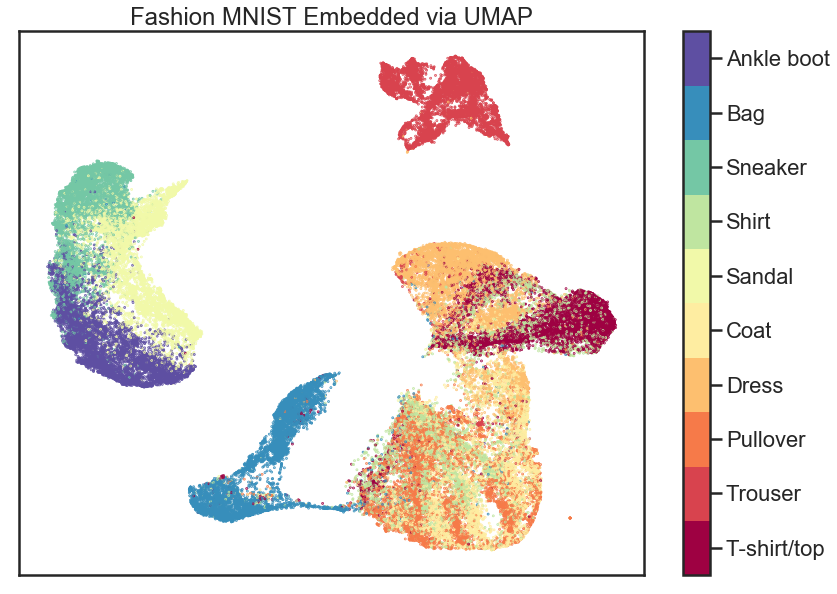
\includegraphics[height=70mm, width=110mm]{umap.png}
	}
	\caption{Алгоритм UMAP}
	\label{figCurves}
\end{figure} 

Получить два новых признака из исходных можно очень многими способами. Но они должны описывать выборку как можно лучше, чтобы при визуализации мы видели не случайно нарисованное изображение, а отображение начального пространства.

Именно тут пригодится кросс-энтропия, но начнем немного издалека. В UMAP используется дивергенция Кульбака-Лейблера для случайной величины Бернулли $X \sim B(p(x))$. Здесь $p(x)$ --- некоторая функция, определяющая вероятность того, что $X=1$. Запишем формулу $D_{KL}$ для $X$:
\[D_{KL}(P\, ||\, \tilde P)= - p(x)\log \tilde p(x) - (1 - p(x))\log (1 - \tilde p(x)) + p(x)\log p(x) + (1 - p(x))\log (1 - p(x)) = \]
\[= p(x)\log \frac{p(x)}{\tilde p(x)} + (1 - p(x))\log \frac{1 - p(x)}{1 - \tilde p(x)}\]

Однако алгоритм рассчитывает не просто разницу между двумя распределениями для одной случайной величины, а сумму таких разниц для $n$ случайных величин:
\[C_P(\tilde P) = \sum_{i=1}^n p(x_i)\log \frac{p(x_i)}{\tilde p(x_i)} + (1 - p(x_i))\log \frac{1 - p(x_i)}{1 - \tilde p(x_i)}\]

Данная величина показывает степень отдаленности друг от друга множеств из случайных величин: $P$ и $\tilde P$. При этом каждому множеству соответствует своя функция: $p(x)$ и $\tilde p(x)$. 

Минимизация $C_P(\tilde P)$ по $\tilde p(x)$ позволяет найти множество $\tilde P$, которое наиболее похоже на множество $P$.

Задача минимизации заключается в поиске оптимального $\tilde p(x)$. Если вернуться к исходной записи $D_{KL} = H_p(\tilde{p}) - H(p)$, то видно, что энтропия не зависит от $\tilde p(x)$, соответственно, является константой при минимизации. Тогда задача преобразуется в оптимизацию лишь суммы кросс-энтропий:
\[- \sum_{i=1}^n \left(p(x_i)\log \tilde p(x_i) + (1 - p(x_i))\log (1 - \tilde p(x_i))\right) \rightarrow \min_{\tilde p}\]

Поэтому UMAP считается методом, основанным на кросс-энтропии.

При отображении пространстве UMAP строит взвешенный граф из объектов. Веса ребер можно воспринимать как вероятность существования данного ребра. Поэтому ребро $e$ является случайной величиной, имеющей распределение Бернулли: $e \sim B(w(e))$, где $w(e)$ --- вес ребра $e$. Получается, что множество ребер построенного графа --- множество $E$ из случайных величин Бернулли.

Тогда для более корректного переноса данных мы можем подобрать для множества~$E_h$ похожее на него множество~$E_l$ с функцией~$w_l(e)$, соответствующие низкоразмерному пространству.

Например, пусть у нас есть выборка из 3 объектов, и мы знаем веса ребер между ними в исходном пространстве:
\begin{center}
	\begin{tabular}{|c||c|c|c|}
		\hline
		& D & Y & L\\
		\hline
		\hline
		D & - & 0.7 & 0.1\\
		\hline
		Y & 0.7 & - & 0.3\\
		\hline
		L & 0.1 & 0.3 & -\\
		\hline
	\end{tabular}
\end{center}

UMAP выполняет автоматическую минимизацию кросс-энтропии. Поскольку вручную данное действие выполнить сложно, то мы можем попробовать подобрать $t(m)$ с наименьшей дивергенцией Кульбака-Лейблера, выбирая из нескольких множеств:

\begin{center}
	\begin{multicols}{2}
		\begin{tabular}{|c||c|c|c|}
			\hline
			$t_1$ & D & Y & L\\
			\hline
			\hline
			D & - & 0.6 & 0.3\\
			\hline
			Y & 0.6 & - & 0.5\\
			\hline
			L & 0.3 & 0.5 & -\\
			\hline
		\end{tabular}\\
		\begin{tabular}{|c||c|c|c|}
			\hline
			$t_2$ & D & Y & L\\
			\hline
			\hline
			D & - & 0.1 & 0.9\\
			\hline
			Y & 0.1 & - & 0.4\\
			\hline
			L & 0.9 & 0.4 & -\\
			\hline
		\end{tabular}
	\end{multicols}
\end{center}

Кросс-энтропия для $t_1(m)$:
\[C_{E_h}(E_l)_1 = 0.7\log \frac{0.7}{0.6} + (1-0.7)\log \frac{1-0.7}{1-0.6} + 0.1\log \frac{0.1}{0.3} + (1-0.1)\log \frac{1-0.1}{1-0.3}+\] \[+ 0.3\log \frac{0.3}{0.5} + (1-0.3)\log \frac{1-0.3}{1-0.5} \approx 0.22\]

Кросс-энтропия для $t_2(m)$:
\[C_{E_h}(E_l)_2 = 0.7\log \frac{0.7}{0.1} + (1-0.7)\log \frac{1-0.7}{1-0.1} + 0.1\log \frac{0.1}{0.9} + (1-0.1)\log \frac{1-0.1}{1-0.9} +\]\[+ 0.3\log \frac{0.3}{0.4} + (1-0.3)\log \frac{1-0.3}{1-0.4} \approx 2.81\]

Так как наша цель --- минимальная дивергенция Кульбака-Лейблера, то множество весов с функцией $t_1(m)$ подходит для решения задачи больше, чем $t_2$. Вероятно, можно подобрать еще более оптимальное множество, однако проще доверить эту работу UMAP.


\end{document}
